\section{Introduction and Motivation}
\label{sec:intro}

The Scottish COVID-19 Response Consortium (SCRC) \cite{2020University}, in collaboration with the Royal Society's call to action in March 2020, has taken a proactive approach to address the need for enhanced epidemiological models of COVID-19 transmission.
This joint volunteer effort, known as Rapid Assistance in Modelling the Pandemic (RAMP) \cite{2020Rapid}, aims to foster a deeper comprehension of the consequences associated with various exit strategies from lockdown measures.
Moreover, this consortium attracted the involvement of distinguished scientists and experts from diverse organizations both within the United Kingdom and abroad, thus augmenting the collective knowledge base and ensuring comprehensive expertise in specialized domains.

RAMPVis \cite{2020Visualization} is a group of researchers specialized in Data Visualization and Visual Analytics (abbreviated as VIS).
This group voluntarily came forward to contribute its specialized skills and knowledge in order to provide valuable support to the SCRC modelers.
The term \textit{modelers} used here refers to the SCRC researchers who were actively engaged in the development of epidemiological models at SCRC.
This predominantly includes experts in domains such as mathematics, statistics, and epidemiology.

Serving as the volunteer team responsible for providing visualization support to one of the six epidemiological models developed by the SCRC modelers \cite{chen2022RAMPVIS}, our main objective is to provide VIS researchers and practitioners with valuable insights gained from our research and development (R\&D) activities conducted during the COVID-19 pandemic.
In an effort to predict the potential impact of diverse interventions, modelers have actively utilized COVID-19 data, employing a method known as Uncertainty Quantification (UQ).
This process seeks to measure uncertainties through the application of mathematical models and simulations.
However, modelers are faced with significant challenges, including the aspects of expert elicitation and effective communication.
In other words, there is a need for software engineering effort coupled with visualization to provide support for the validation and verification tests, and to create efficient workflows between modelers and researchers from other disciplines \cite{ackland2022Royal}.

\begin{figure}[tb!]
    \centering
    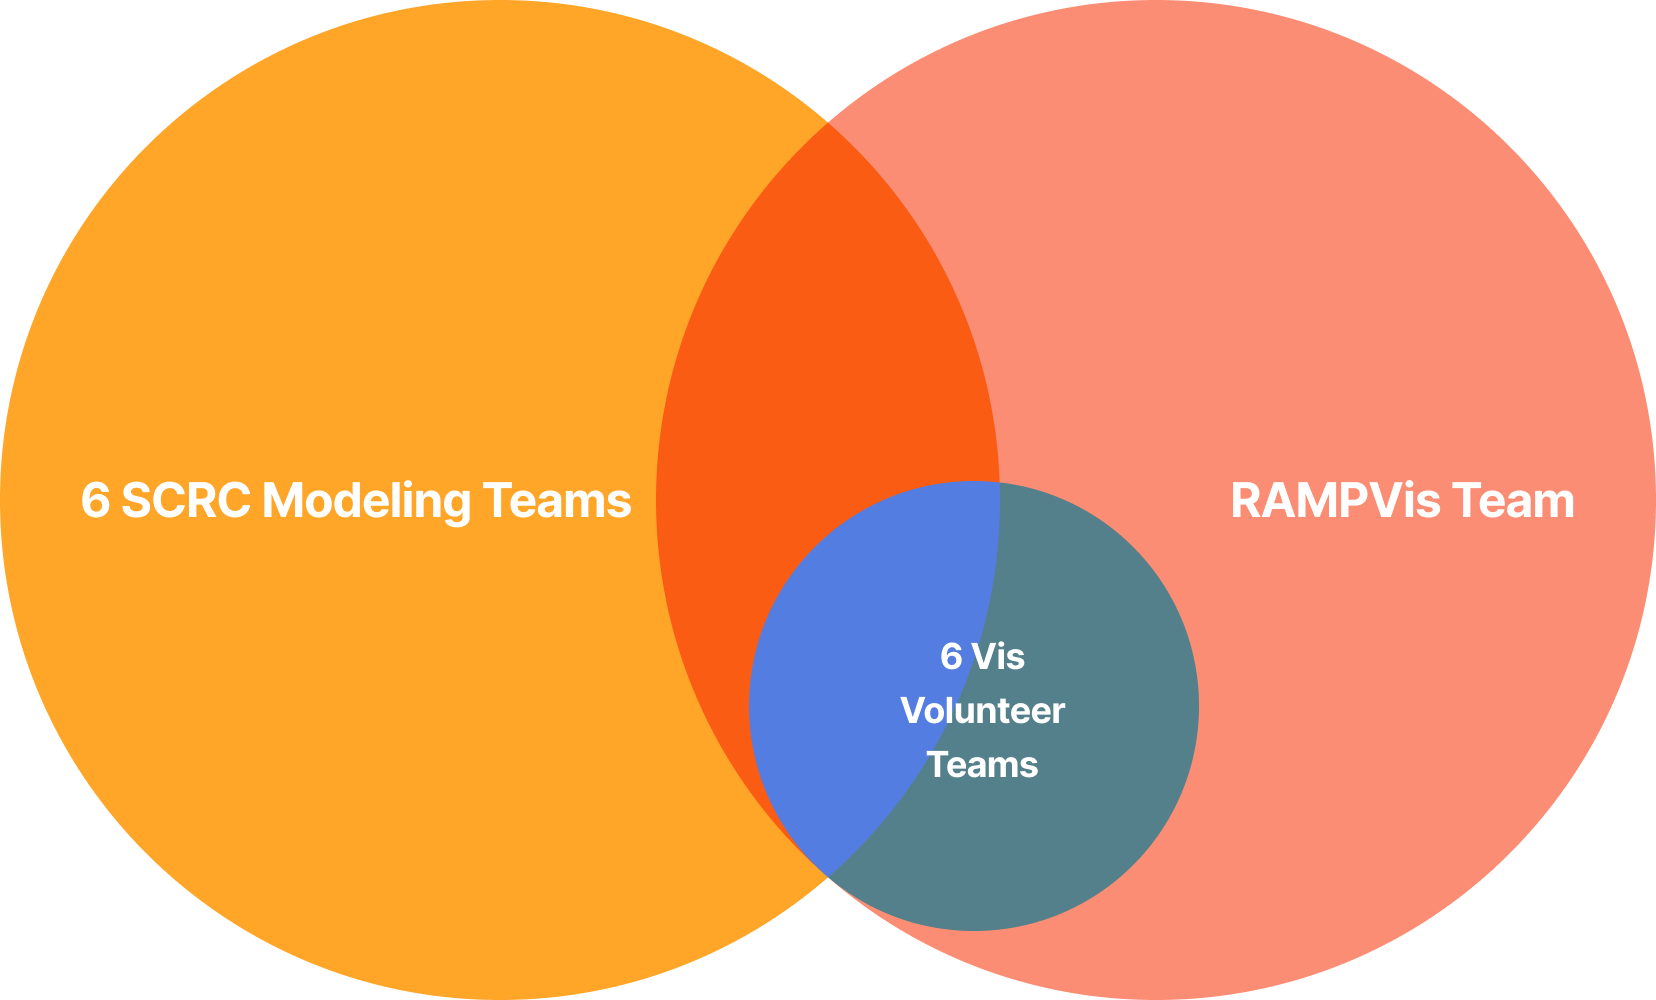
\includegraphics[width=0.75\linewidth]{venn.png}
    \caption{The organization of researchers from the SCRC and RAMPVis. The 6 SCRC modeling team are responsible for developing the epidemiological models leveraging different modeling techniques. The RAMPVis team provides visualization support to the SCRC modeling team, by establishing 6 VIS volunteer teams who work on the actual development under the guidance of the RAMPVis team.
    }
    \label{fig:venn}

\end{figure}

In addressing these hurdles, \ac{VIS} emerge as a potent tool, offering the capacity to significantly enhance and streamline their collaborative workflows \cite{swallow2022Challenges}.
While our work may not have showcased the state-of-the-art VIS techniques, it effectively delivered rapid and practical VIS support to the modelers during an exceptional and demanding time.
The exemplification of a fully virtual collaboration among researchers from various UK institutions epitomizes the spirit of interdisciplinary cooperation in response to the pandemic.

What we present here is an early history of our volunteer response from a software and visualization perspective. We present the earliest stages of visualization dashboard, EnsembleDashVis, developed from 2020, aiming to assist the modelers in intrepreting an \ac{ABC-SMC} inference model that they have developed using COVID-19 data collected during the first wave of the outbreak in Scotland \cite{2020Covid19}. Much of this effort and the reasoning behind this volunteer was never documented.
